\documentclass[border=6pt]{standalone}
% Shared preamble for web figures.  Each figure is a standalone .tex that
% \input's this file; scripts/make-figures.sh turns it into an SVG.
% Handouts pull the same file with \fig{Unit_X/<name>}.
\usepackage[T1]{fontenc}
\usepackage{helvet}
\renewcommand{\familydefault}{\sfdefault}
\renewcommand{\ttdefault}{pcr}  % Courier: a real Type 1 typewriter font
\usepackage{amsmath}
\usepackage{tikz}
\usetikzlibrary{arrows.meta,positioning,calc,shapes.symbols,shapes.geometric}

% Who makes the rules is the point of most diagrams in this book, so the
% colors mean the same thing everywhere: blue is a person, orange is the
% computer, green is an answer, pink is the human brain.
\definecolor{person}{HTML}{2C6FAE}
\definecolor{machine}{HTML}{D35400}
\definecolor{result}{HTML}{1E8449}
\definecolor{brainpink}{HTML}{C2185B}
\definecolor{ink}{HTML}{2C3E50}

\tikzset{
  doodle/.style={line width=1.5pt, line cap=round, line join=round, draw=ink},
  box/.style={draw, rounded corners=5pt, line width=1.1pt, align=center,
              inner sep=7pt, minimum height=1.0cm, font=\small},
  personbox/.style={box, draw=person, fill=person!10},
  machinebox/.style={box, draw=machine, fill=machine!10},
  resultbox/.style={box, draw=result, fill=result!10},
  plainbox/.style={box, draw=ink!70, fill=ink!4},
  flow/.style={-{Stealth[length=8pt]}, line width=1.4pt, draw=ink},
}

% A person (blue) and a robot head (orange) as small icons.
% \personicon{x}{y}{scale}   \roboticon{x}{y}{scale}
\newcommand{\personicon}[3]{%
  \begin{scope}[shift={(#1,#2)}, scale=#3]
    \fill[person] (0,0.62) circle (0.28);
    \fill[person, rounded corners=6pt] (-0.42,-0.55) rectangle (0.42,0.28);
  \end{scope}}
\newcommand{\roboticon}[3]{%
  \begin{scope}[shift={(#1,#2)}, scale=#3]
    \draw[machine, line width=1.2pt] (0,0.5) -- (0,0.72);
    \fill[machine] (0,0.78) circle (0.08);
    \draw[machine, line width=1.4pt, fill=machine!12, rounded corners=4pt] (-0.5,-0.45) rectangle (0.5,0.5);
    \fill[ink] (-0.2,0.12) circle (0.08);
    \fill[ink] (0.2,0.12) circle (0.08);
    \draw[ink, line width=1pt] (-0.22,-0.22) -- (0.22,-0.22);
  \end{scope}}

\begin{document}
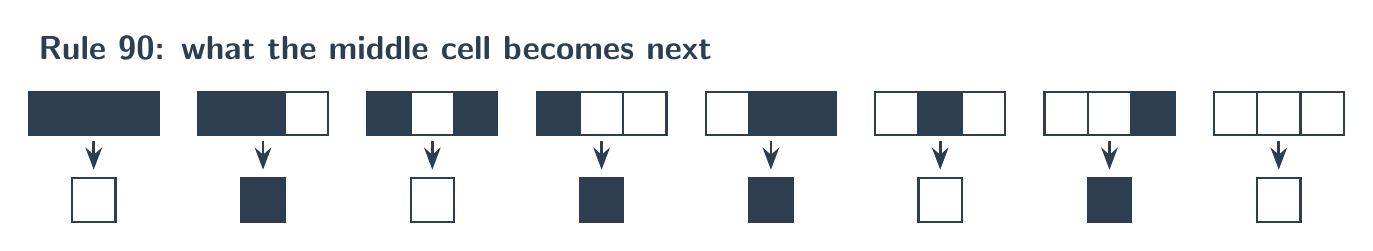
\begin{tikzpicture}

% The Rule 90 card: for each 3-cell pattern, the color of the middle cell next.

\draw[ink, line width=0.8pt, fill=ink] (0.000,1.1) rectangle ++(0.55,0.55);
\draw[ink, line width=0.8pt, fill=ink] (0.550,1.1) rectangle ++(0.55,0.55);
\draw[ink, line width=0.8pt, fill=ink] (1.100,1.1) rectangle ++(0.55,0.55);
\draw[flow, line width=1pt] (0.825,1.02) -- (0.825,0.66);
\draw[ink, line width=0.8pt, fill=white] (0.550,0) rectangle ++(0.55,0.55);
\draw[ink, line width=0.8pt, fill=ink] (2.150,1.1) rectangle ++(0.55,0.55);
\draw[ink, line width=0.8pt, fill=ink] (2.700,1.1) rectangle ++(0.55,0.55);
\draw[ink, line width=0.8pt, fill=white] (3.250,1.1) rectangle ++(0.55,0.55);
\draw[flow, line width=1pt] (2.975,1.02) -- (2.975,0.66);
\draw[ink, line width=0.8pt, fill=ink] (2.700,0) rectangle ++(0.55,0.55);
\draw[ink, line width=0.8pt, fill=ink] (4.300,1.1) rectangle ++(0.55,0.55);
\draw[ink, line width=0.8pt, fill=white] (4.850,1.1) rectangle ++(0.55,0.55);
\draw[ink, line width=0.8pt, fill=ink] (5.400,1.1) rectangle ++(0.55,0.55);
\draw[flow, line width=1pt] (5.125,1.02) -- (5.125,0.66);
\draw[ink, line width=0.8pt, fill=white] (4.850,0) rectangle ++(0.55,0.55);
\draw[ink, line width=0.8pt, fill=ink] (6.450,1.1) rectangle ++(0.55,0.55);
\draw[ink, line width=0.8pt, fill=white] (7.000,1.1) rectangle ++(0.55,0.55);
\draw[ink, line width=0.8pt, fill=white] (7.550,1.1) rectangle ++(0.55,0.55);
\draw[flow, line width=1pt] (7.275,1.02) -- (7.275,0.66);
\draw[ink, line width=0.8pt, fill=ink] (7.000,0) rectangle ++(0.55,0.55);
\draw[ink, line width=0.8pt, fill=white] (8.600,1.1) rectangle ++(0.55,0.55);
\draw[ink, line width=0.8pt, fill=ink] (9.150,1.1) rectangle ++(0.55,0.55);
\draw[ink, line width=0.8pt, fill=ink] (9.700,1.1) rectangle ++(0.55,0.55);
\draw[flow, line width=1pt] (9.425,1.02) -- (9.425,0.66);
\draw[ink, line width=0.8pt, fill=ink] (9.150,0) rectangle ++(0.55,0.55);
\draw[ink, line width=0.8pt, fill=white] (10.750,1.1) rectangle ++(0.55,0.55);
\draw[ink, line width=0.8pt, fill=ink] (11.300,1.1) rectangle ++(0.55,0.55);
\draw[ink, line width=0.8pt, fill=white] (11.850,1.1) rectangle ++(0.55,0.55);
\draw[flow, line width=1pt] (11.575,1.02) -- (11.575,0.66);
\draw[ink, line width=0.8pt, fill=white] (11.300,0) rectangle ++(0.55,0.55);
\draw[ink, line width=0.8pt, fill=white] (12.900,1.1) rectangle ++(0.55,0.55);
\draw[ink, line width=0.8pt, fill=white] (13.450,1.1) rectangle ++(0.55,0.55);
\draw[ink, line width=0.8pt, fill=ink] (14.000,1.1) rectangle ++(0.55,0.55);
\draw[flow, line width=1pt] (13.725,1.02) -- (13.725,0.66);
\draw[ink, line width=0.8pt, fill=ink] (13.450,0) rectangle ++(0.55,0.55);
\draw[ink, line width=0.8pt, fill=white] (15.050,1.1) rectangle ++(0.55,0.55);
\draw[ink, line width=0.8pt, fill=white] (15.600,1.1) rectangle ++(0.55,0.55);
\draw[ink, line width=0.8pt, fill=white] (16.150,1.1) rectangle ++(0.55,0.55);
\draw[flow, line width=1pt] (15.875,1.02) -- (15.875,0.66);
\draw[ink, line width=0.8pt, fill=white] (15.600,0) rectangle ++(0.55,0.55);
\node[anchor=west, font=\large\bfseries, text=ink] at (0,2.2) {Rule 90: what the middle cell becomes next};
\end{tikzpicture}
\end{document}
